\documentclass[conference,a4paper]{IEEEtran}
\usepackage{graphicx}
\usepackage{amsmath}
\usepackage{booktabs}
\usepackage{cite}
\usepackage{url}
\pagestyle{empty}

\newcommand{\refpending}{\textbf{[ref.\ pending]}}

\begin{document}

\title{Crop Allocation as a QUBO: Constraint Encoding,\\Solver Choice, and the Agricultural Cost of Occupation}

\author{\IEEEauthorblockN{Anonymous Submission}
\IEEEauthorblockA{NGIA-QC 2026 --- Double-blind review}}

\maketitle
\thispagestyle{empty}

\begin{abstract}
When many farmers independently choose the same profitable crop, the
combined harvest depresses its price. We formulate the resulting allocation
problem as a 1{,}914-variable QUBO over 174 real parcels (1{,}464~ha) in
Jenin, Palestine, with a Random Forest scoring suitability and irrigation
priced rather than capped. How a discrete choice is encoded in binary
variables is usually treated as an implementation detail. Here it decides the
outcome. In a $2\times2$ benchmark over 20 seeds at a matched wall-clock
budget, domain-wall encoding raises discrete simulated bifurcation's profit by
152\% and brings it level with simulated annealing, yet costs annealing
8.5\%. The encoding advantage therefore depends on the solver's move set,
which single-solver studies cannot reveal. A myopic baseline loses money by
flooding the market, and restricting cultivation to Areas A/B under occupation
costs \$0.23--1.22M/yr within a fixed water budget.
\end{abstract}

\begin{IEEEkeywords}
quantum-inspired optimisation, simulated bifurcation, QUBO, domain-wall
encoding, crop planning, random forest
\end{IEEEkeywords}

\section{Introduction}

Crop planning is an allocation problem constrained by a market signal no
individual farmer can observe. A farmer plants on last season's prices,
without knowing what the neighbours intend; when many independently converge
on the same profitable crop, the combined harvest depresses its price. Each decision is individually rational and the aggregate
outcome is a collective loss, a coordination failure that bites hardest for
perishables, which cannot be stored until prices recover. The northern West
Bank has lived through this repeatedly, including a cucumber glut in 2021 and
a collapse in tomato prices in 2025 \refpending. Recent crop-planning models
therefore treat market absorption as a binding constraint rather than assuming
prices are exogenous to the plan~\cite{li2025,hou2026}.

Allocation in Jenin governorate is shaped by two further constraints, both
consequences of occupation. Under the Oslo interim framework the occupied West
Bank is divided into Areas A and B, administered by the Palestinian Authority,
and Area C, which remains under full Israeli military and administrative
control. Agricultural development in Area C requires permits that are rarely
granted, and more than 70\% of the communities located there have no
connection to the water network~\cite{ochaareac}. In 2024 the International
Court of Justice found Israel's continued presence in the occupied Palestinian
territory unlawful, including its use of the territory's natural
resources~\cite{icj2024}. Within our study window, 32.5\% of the mapped
agricultural parcel area lies in Area C, and irrigation across the remainder
draws on an agricultural water budget of roughly 6.0~Mm$^3$/yr \refpending.
Measuring what these restrictions cost parcel by parcel, rather than through
national accounts~\cite{worldbank2014}, means solving the allocation problem
once under each land regime. The computational question that follows is a
prerequisite, not an aside.

Allocating $P$ parcels among $C$ crops admits $C^P$ candidate assignments, and
the problem does not decompose: because revenue depends on aggregate
production, the best crop for one parcel depends on the choices made for all
the others. Problems of this form map onto quadratic unconstrained binary
optimisation (QUBO)~\cite{lucas2014,glover2019}, the input format shared by
quantum annealers and by a growing family of quantum-inspired classical
solvers. Among the latter, simulated bifurcation (SB)~\cite{goto2021} integrates the
classical Hamiltonian dynamics of nonlinear oscillators. All variables
update simultaneously, so SB parallelises where sequential methods such as
simulated annealing~\cite{kirkpatrick1983} cannot, and it has matched
annealing hardware on large benchmarks~\cite{zeng2024}.

Passing a discrete allocation problem to any such solver first requires an
\emph{encoding}: a representation of each parcel's crop choice in binary
variables, together with a mechanism enforcing that exactly one crop is
selected. The conventional choice, one-hot encoding, imposes this through a
quadratic penalty and leaves invalid assignments reachable. Domain-wall
encoding~\cite{chancellor2019} instead constrains a chain of binaries so that
the requirement holds by construction. Encoding is ordinarily treated as an
implementation detail, subordinate to the choice of solver. On the instance
studied here, it is not.

We study 174 real parcels (1{,}464~ha) in Jenin as a 1{,}914-variable QUBO
with market-clearing prices and priced irrigation water. Our contributions
are fourfold. First, a $2\times2$ encoding-by-solver benchmark over 20 seeds
at a matched wall-clock budget, in which domain-wall encoding raises
discrete simulated bifurcation's profit by 152\% and brings it level with
simulated annealing, while \emph{lowering} annealing's own profit by 8.5\%;
single-solver studies cannot observe that interaction. Second, a QUBO
formulation in which prices fall with aggregate production and irrigation is
priced rather than capped, so that sweeping the charge recovers the water
shadow price. Third, a bounded parcel-level estimate of the agricultural
cost of restricting Palestinian cultivation to Areas A/B under a fixed water
budget. Fourth, because the objective is driven by prices, a test of whether
a learned forecaster beats recent-mean prices as the optimiser's input; an
LSTM does not outperform persistence at this data scale, and we report that
negative result rather than bury it.

\section{Literature Review}
\label{sec:lit}

\subsection{AI-Based Crop Recommendation and Price Forecasting}

Random Forest, an ensemble of bagged decision trees, remains a strong
baseline for tabular agricultural data because it absorbs nonlinear,
heterogeneous features (soil nutrients, pH, temperature, rainfall) without
extensive preprocessing~\cite{breiman2001}. Dey et al.~\cite{dey2024}
reached classification accuracy above 99\% for crop recommendation with
XGBoost on soil and climatic features, but their pipeline stops at
suitability: with no forecasting or allocation stage, a crop flagged
suitable may still be a poor choice if the market is saturated. Saha et al.~\cite{saha2025} went further, combining satellite land mapping,
machine-learning crop recommendation and yield prediction above 95\%
accuracy, and irrigation control; their LSTM forecasts vegetation area
rather than prices, so it cannot signal oversupply before it occurs.

Because the allocation objective is driven by prices, the quality of the price
input matters as much as the optimiser; Li et al.~\cite{li2025} address this by
feeding neural-network forecasts into theirs. Long Short-Term Memory
networks~\cite{hochreiter1997} are widely applied to agricultural price series
for the same purpose. Their benefit is sensitive to record length, and a
governorate-level history offers only a few decades of annual observations per
crop. Whether a learned forecaster improves on a naive baseline at this data
scale is an empirical question rather than a given, and we treat it as one,
evaluating our LSTM against persistence, autoregressive, moving-average and
trend models before any forecast reaches the optimiser.

\subsection{Optimization Approaches: From Classical Methods to Quantum-Inspired Algorithms}

Crop allocation was traditionally posed as linear programming, but recent
work treats it as a nonlinear problem integrating prediction and market
effects. Li et al.~\cite{li2025} combined simulated annealing with a genetic
algorithm (H-SAGA) across 34 plots in northern China, feeding neural-network
price forecasts into the optimizer and constraining production by regional
market-absorption capacity and farm water supply; H-SAGA beat standalone GA,
SA, PSO and ACO by 5--10 percentage points of profit increment. Hou et al.~\cite{hou2026} paired particle swarm optimization
with simulated annealing and Monte Carlo simulation (PSO--SA--MCS), lowering
prices when production exceeds demand, and raised expected profit by 12.6\%
over a baseline PSO at a runtime complexity of $O(N^2\cdot\mathrm{pop})$.
Integrating forecasting, market saturation and resource limits into a single
allocation model is thus well established with classical metaheuristics.

Quantum and quantum-inspired approaches offer a different route. Simulated
bifurcation~\cite{goto2021} derives from a quantum-mechanical model but
simulates \emph{classical} Hamiltonian dynamics, so it runs on conventional
hardware. Zeng et al.~\cite{zeng2024} benchmarked quantum-annealing-inspired
algorithms, SB among them, against a D-Wave annealer on Max-Cut instances of
up to 20{,}000 nodes: ballistic SB cut time-to-solution nearly fifty-fold on
small and Chimera-structured graphs, and discrete SB was fastest on large
ones. On dense QUBO
instances, Kim et al.~\cite{kim2025} found a hybrid quantum-annealing solver
roughly 6{,}561$\times$ faster than the best classical solver, with marginally
higher accuracy. Within agriculture, Verma et al.~\cite{verma2025} proposed
HQOMLF, pairing a quantum convolutional neural network for prediction with the
Quantum Approximate Optimization Algorithm for resource allocation, and
reported speed-ups of up to 3.5$\times$.

Two gaps remain. First, none of these agricultural studies formulates
allocation as a QUBO with market-clearing prices for Ising-type solvers: Li et
al.\ and Hou et al.\ use classical metaheuristics, and Verma et al.\ apply
QAOA without a market model. Second, the benchmarking literature compares
\emph{solvers}, yet results on a real problem also depend on how constraints
are \emph{encoded}. One-hot encoding enforces one crop per parcel through a
penalty, leaving invalid assignments reachable; Chancellor's domain-wall
encoding~\cite{chancellor2019} makes them unreachable by construction. Chen et
al.~\cite{chen2021} compared the two on D-Wave annealing hardware across three
problems and found domain-wall superior on every metric, with none favouring
one-hot. Berwald et al.~\cite{berwald2022} showed that domain-wall dynamics
freeze later, and conjectured that the advantage extends to gate-model and
quantum-inspired algorithms. That conjecture has not been tested on a
quantum-inspired solver, nor on a real allocation problem. We test it here and
find that it holds only conditionally: large for simulated bifurcation, but
reversed in sign for simulated annealing. Table~\ref{tab:lit} summarizes the
studies reviewed.

\begin{table*}[t]
\centering
\caption{Summary of reviewed studies across crop recommendation, forecasting, and optimization}
\label{tab:lit}
\footnotesize
\begin{tabular}{p{2.5cm}p{3.0cm}p{3.9cm}p{6.6cm}}
\toprule
Study & Focus area & Method & Limitation relative to this study \\
\midrule
Breiman~\cite{breiman2001} & Ensemble learning, general & Random Forest (foundational) & Not agricultural; the method applied here to crop suitability \\
Hochreiter \& Schmidhuber~\cite{hochreiter1997} & Sequence modeling, general & LSTM (foundational) & Not agricultural; the method applied here to price forecasting \\
Dey et al.~\cite{dey2024} & Crop recommendation & XGBoost on soil/climate features & Suitability only; no forecasting or allocation stage \\
Saha et al.~\cite{saha2025} & Land suitability, irrigation & ML + LSTM (vegetation), satellite data & LSTM forecasts vegetation area, not prices; no allocation stage \\
Li et al.~\cite{li2025} & Dynamic multi-plot crop planning & Hybrid SA--GA + neural-network price forecasts & Classical metaheuristic; no QUBO or encoding analysis; no land restrictions \\
Hou et al.~\cite{hou2026} & Crop planning under uncertainty & Hybrid PSO--SA + Monte Carlo & No learned forecasts; classical metaheuristic \\
Zeng et al.~\cite{zeng2024} & Quantum-inspired optimization & SB and simulated CIM vs.\ D-Wave annealer & Abstract Max-Cut benchmarks; compares solvers, not encodings \\
Kim et al.~\cite{kim2025} & Large-scale dense QUBO & Hybrid quantum annealing vs.\ classical solvers & Benchmark instances; compares solvers, not encodings \\
Verma et al.~\cite{verma2025} & Quantum computing in precision agriculture & QCNN + QAOA (HQOMLF) & No market-clearing prices; no encoding analysis; no SB comparison \\
Chancellor~\cite{chancellor2019} & Encoding discrete variables & Domain-wall encoding & Theoretical; not evaluated on a real-world allocation problem \\
Chen et al.~\cite{chen2021} & Encoding comparison, experimental & Domain-wall vs.\ one-hot on D-Wave hardware & Annealing hardware, abstract problems; one solver class, so the interaction
is unobservable \\
Berwald et al.~\cite{berwald2022} & Encoding theory and dynamics & Variable-count optimality; freezing behaviour & Conjectures the extension to quantum-inspired solvers, untested \\
\bottomrule
\end{tabular}
\end{table*}

Integrated crop planning combining prediction, market saturation and
resource limits is thus established with classical
metaheuristics~\cite{li2025,hou2026}, and quantum-inspired solvers perform
strongly on abstract benchmarks~\cite{zeng2024,kim2025}. What remains
unexamined is where the two meet: agricultural allocation as a QUBO with
market-clearing prices, and the effect of encoding on the solvers that
consume it. We address that gap on 174 real parcels in Jenin, under the land
and water restrictions specific to the occupied West Bank.

%% ============================================================
%% METHODOLOGY -- REMOVED FOR TALA TO WRITE.
%% Reference text: METHODOLOGY_REMOVED.tex
%% Requirements:   METHODOLOGY_BRIEF.md
%% ============================================================
\section{Methodology}
\label{sec:method}

\textit{[This section is to be written. It must cover: study area and
data sources; the Random Forest suitability model; the QUBO formulation;
and the two encodings and two solvers compared, including the matched
wall-clock protocol. See METHODOLOGY\_BRIEF.md for every number the
Results section depends on.]}

\section{Results}
\label{sec:results}

\subsection{Suitability and Price Forecasting}

In 5-fold stratified cross-validation the Random Forest reaches
$0.9945\pm0.0037$ accuracy on real data against a majority-class baseline of
0.0455, and $0.8514\pm0.0291$ on synthetic EcoCrop rows, which measures
fidelity to the envelopes rather than predictive skill. Feature
importances are rainfall 0.251, humidity 0.192, K 0.166, P 0.139, N 0.098,
temperature 0.082 and pH 0.072, so the unmeasured P and K together carry
30.5\%. Under Jenin's inputs the model gives oranges zero probability on every
parcel, and oranges are consequently never assigned.

The optimiser requires a price for each crop. To decide whether that price
should be forecast or taken from recent history, we compared an
LSTM~\cite{hochreiter1997} of 24 hidden units and 3{,}481 parameters against
four naive baselines (Table~\ref{tab:lstm}). The LSTM was trained on pooled
log-price windows with augmentation applied to training data only, under
walk-forward validation with the split made before normalisation.

\begin{table}[t]
\centering
\caption{Price forecasts, 50 test windows, 2024 excluded}
\label{tab:lstm}
\footnotesize
\begin{tabular}{lcc}
\toprule
Model & RMSE (\$/t) & MAPE (\%) \\
\midrule
\textbf{Persistence} & \textbf{130.1} & \textbf{16.3} \\
AR(1) & 150.5 & 18.3 \\
Mean of last 3 & 170.1 & 19.7 \\
Linear trend & 186.0 & 20.9 \\
LSTM (pooled, augmented) & 252.2 & 26.7 \\
\bottomrule
\end{tabular}
\end{table}

The LSTM ranks last. With 142 training windows drawn from 13--27 annual
observations per crop, 3{,}481 parameters are not constrained, and
augmentation adds no information the series does not already contain. The
optimisation therefore uses 2019--2023 mean prices. Including 2024 in the test
window reverses the ranking (LSTM RMSE 624.2 against 639.6 for persistence),
but the wartime shock raises persistence error 4.9-fold and LSTM error only
2.5-fold, so a window containing 2024 rewards robustness to a discontinuity
rather than forecasting skill.

\subsection{Encoding Versus Solver}

\begin{table}[t]
\centering
\caption{Encoding by solver, 20 seeds, 2.5\,s per run}
\label{tab:bench}
\footnotesize
\setlength{\tabcolsep}{4pt}
\begin{tabular}{llcccc}
\toprule
Enc. & Solver & Profit (M\$) & Invalid & Unsuit. & Water (Mm$^3$) \\
\midrule
one-hot & SA  & $5.42\pm0.26$ & 0.0   & 0.5  & 5.48 \\
one-hot & dSB & $1.98\pm0.42$ & 129.1 & 10.7 & 2.20 \\
dom.-wall & SA  & $4.97\pm0.39$ & 13.0 & 0.3 & 6.25 \\
dom.-wall & dSB & $5.00\pm0.30$ & 2.9  & 0.0 & 5.97 \\
\midrule
\multicolumn{2}{l}{Greedy} & $-1.58$ & --- & 0 & 5.98 \\
\bottomrule
\end{tabular}
\end{table}

\begin{figure}[t]
\centering
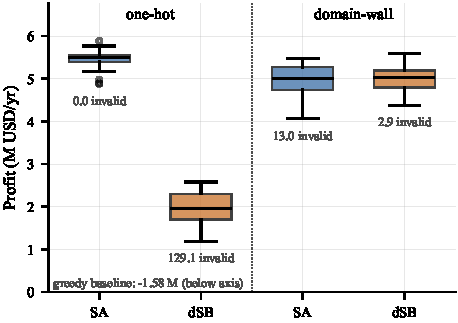
\includegraphics[width=\columnwidth]{figures/fig_encoding.pdf}
\caption{Profit over 20 seeds, with the mean number of parcels holding an
invalid assignment.}
\label{fig:encoding}
\end{figure}

Table~\ref{tab:bench} and Fig.~\ref{fig:encoding} give the results, where
``Invalid'' counts parcels whose binary block is not a valid assignment.
Under one-hot encoding dSB leaves 129 of 174 parcels invalid and earns 63\%
less than SA ($p<10^{-7}$): its continuous dynamics bifurcate variables
independently, and the dense per-parcel penalty does not reliably leave
exactly one positive. Domain-wall encoding raises dSB profit by 152\%
($p<10^{-7}$), after which the two solvers do not differ (dSB $+0.6\%$,
$p=0.93$).

The encoding effect is not symmetric. Domain-wall \emph{lowers} SA profit by
8.5\% ($p<10^{-4}$) and leaves SA with 13 invalid parcels, because the
ordering penalty is not sized to SA's single-bit moves. This is a metric on
which one-hot performs better, which Chen et al.~\cite{chen2021} did not
observe on annealing hardware. The encoding advantage appears to depend on the
solver's move set, so the conjecture of Berwald et al.~\cite{berwald2022}
holds for bifurcation dynamics but not for single-bit annealing. The best
configuration overall remains classical SA with one-hot encoding. Our finding
is that encoding choice decides whether the quantum-inspired solver is usable
at all, not that it outperforms annealing.

The greedy plan loses \$1.58M. Assigning every parcel its best-margin crop
concentrates production in a few crops far beyond $D_j$. Even when unsaleable
surplus is discarded rather than sold at the negative prices a linear demand
curve implies beyond $2D_j$, it still loses \$1.55M. This is the glut
mechanism that motivates the study.

\subsection{Water Shadow Price and the Cost of Land Restriction}

\begin{figure}[t]
\centering
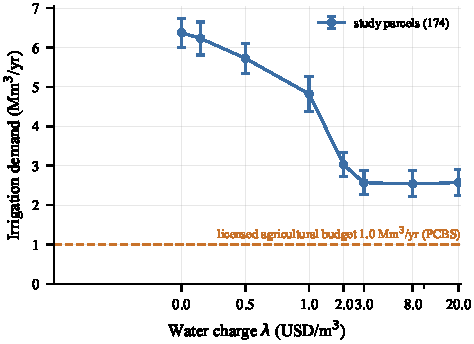
\includegraphics[width=\columnwidth]{figures/fig_water.pdf}
\caption{Irrigation demand against the water charge $\lambda$ (SA, one-hot,
10 seeds; bars are one standard deviation).}
\label{fig:water}
\end{figure}

Sweeping $\lambda$ traces the demand for irrigation water
(Fig.~\ref{fig:water}). Restricted to Areas A/B, demand peaks at
5.50~Mm$^3$/yr, so the 6.0~Mm$^3$ budget never binds and its shadow price is
zero. Across the full land base at the same market size, demand reaches
7.96~Mm$^3$ and the budget binds at \$1.09/m$^3$, or \$1.35/m$^3$ if the
market grows with land. Water scarcity in Jenin is a consequence of land
restriction, not an independent limit.

\begin{table}[t]
\centering
\caption{Cost of restricting cultivation, within the 6.0\,Mm$^3$ water budget}
\label{tab:areac}
\footnotesize
\setlength{\tabcolsep}{4pt}
\begin{tabular}{lccc}
\toprule
Land regime & Area (ha) & Profit (M\$/yr) & Loss \\
\midrule
Full land base, market fixed & 2{,}169 & 5.59 & --- \\
Full land base, market $\times1.48$ & 2{,}169 & 6.58 & --- \\
Restricted to Areas A/B & 1{,}464 & 5.36 & 0.23--1.22 \\
\bottomrule
\end{tabular}
\end{table}

Table~\ref{tab:areac} compares land regimes at identical prices, yields,
suitability thresholds and water budget. Confining cultivation to Areas A/B
withholds 706~ha and costs \$0.23M/yr at the present market size, or
\$1.22M/yr if unrestricted access brought proportionate market access. The
range is wide because, with water binding and a fixed market, extra land
mostly adds supply that cannot be sold at a profit: the value of land access
depends on market access, and occupation restricts both. On SoilGrids
estimates, Area C and A/B parcels are similar in pH (7.69 vs.\ 7.71), clay
(46.2 vs.\ 46.4\%) and cation exchange capacity (34.2 vs.\ 36.0~cmol/kg), and
Area C carries higher soil organic carbon (28.3 vs.\ 20.7~g/kg). Nothing in
these estimates suggests the withheld land is poorer.

\subsection{Price Robustness}

The optimum is degenerate: inverse demand equalises marginal revenue across
crops, so many parcel-level plans reach similar profit, and two baseline runs
differing only in seed agree on just 18.4\% of parcels. Parcel-level agreement
is therefore uninformative, and we compare crop mix by area instead, as
$1-$ total variation distance, against a seed-control floor (10 seeds each).

\begin{table}[t]
\centering
\caption{Crop-mix similarity to the baseline plan}
\label{tab:robust}
\footnotesize
\begin{tabular}{lcc}
\toprule
Scenario & Profit (M\$/yr) & Mix similarity \\
\midrule
\emph{Seed control} & \emph{5.12} & \emph{93.0\%} \\
LSTM prices / persistence & 4.96 / 4.93 & 93.0 / 93.7\% \\
Uniform $-15\%$ / $+15\%$ & 3.20 / 7.41 & 90.6 / 93.2\% \\
Uniform $+30\%$ / perish.\ $+30\%$ & 9.80 / 8.86 & 91.6 / 92.1\% \\
Uniform $-30\%$ / perish.\ $-30\%$ & 1.45 / 2.38 & 84.6 / 84.4\% \\
\bottomrule
\end{tabular}
\end{table}

Every moderate scenario, the LSTM and persistence price vectors included, lies
within 2.4 points of the seed-control floor. Only a 30\% price fall shifts the
crop mix beyond that, moving land toward grapes, olives, wheat and fallow.

\section{Limitations}
\label{sec:limits}

Market size $D_j$ is an assumption, which is why we report the cost of land
restriction as a range rather than a point estimate. The linear demand curve
carries no meaning beyond $Q_j=2D_j$. Climate comes from a single grid cell;
phosphorus and potassium are sampled, not measured; available nitrogen and
irrigation requirements are approximations; SoilGrids values are model
estimates, not field measurements. Yields are national series rescaled to
regional open-field levels, with tree crops assumed at steady bearing. We did not tune the domain-wall ordering penalty, so the 8.5\% annealing
penalty is an upper bound on that encoding's true cost. OpenStreetMap under-
represents unmapped smallholdings. At 1{,}914 variables with ten 174-node
cliques, the instance also exceeds the largest fully connected problem
directly embeddable on current annealing hardware ($K_{150}$ on
Pegasus~\cite{dwaveembed}), though hybrid solvers~\cite{kim2025} could
accept it.

\section{Conclusion}
\label{sec:concl}

On a real 1{,}914-variable crop-allocation QUBO, encoding choice decided
whether a quantum-inspired solver was usable. Domain-wall encoding raised
discrete simulated bifurcation's profit by 152\% and brought it level with
simulated annealing, while costing annealing 8.5\%. The domain-wall advantage
reported on annealing hardware~\cite{chen2021} therefore does not transfer
unconditionally to quantum-inspired solvers: it depends on the solver's move
set, and we identify a case in which one-hot is the better encoding. A myopic
greedy plan lost money by flooding the market, which is the failure that
market-aware allocation exists to prevent. For Jenin, irrigation water does
not bind on the land Palestinian farmers are currently permitted to use, and
confining cultivation to Areas A/B costs \$0.23--1.22M/yr within the water
budget, depending on market access. Future work should tune the domain-wall
ordering penalty, measure freezing behaviour in both solvers to test the
mechanism proposed by Berwald et al.~\cite{berwald2022}, obtain crop-level
demand data, and extend the model to multi-season rotations.

{\footnotesize
\bibliographystyle{IEEEtran}
\bibliography{references}
}

\end{document}
